\RequirePackage[T1]{fontenc}
\documentclass[12pt]{article}

\usepackage[height=8.85in,width=6.45in]{geometry}
%\usepackage{showkeys}
\renewcommand{\baselinestretch}{1.08}

\usepackage[utf8]{inputenc}
\usepackage{amsmath}
\usepackage{amssymb}
\usepackage{mathtools}
\numberwithin{equation}{section}
\usepackage{slashed}
\usepackage{braket}
\usepackage[svgnames]{xcolor}
\usepackage[colorlinks,citecolor=DarkGreen,linkcolor=FireBrick,urlcolor=FireBrick,linktocpage,unicode]{hyperref}
\urlstyle{rm}
\usepackage{cite}
\usepackage{graphicx}
\usepackage{tikz}
\usepackage{tikz-cd}
\usepackage{times}
\usepackage{courier}
\usepackage{bm}
\usepackage{subfig}
\usepackage{ascmac}
\usepackage{spectralsequences}
\usepackage{dashbox}

\DeclareSseqGroup\tower {} {
	\class(0,0)\foreach \i in {1,...,8} {
		\class(0,\i)
		\structline(0,\i-1,-1)(0,\i,-1)
	}
}

\usepackage{xcolor}
\usepackage{colortbl}
\usepackage{arydshln}
\definecolor{lightyellow}{rgb}{1.0, 0.95, 0.7}
\definecolor{blue}{rgb}{0.0, 0.4, 1.0}
\definecolor{Blue}{rgb}{0,0,1}
\definecolor{darkgreen}{rgb}{0.,0.6,0.}
\newcommand*{\red}[1]{\textcolor{red}{#1}}
\newcommand*{\Blue}[1]{\textcolor{Blue}{#1}}
\newcommand*{\blue}[1]{\textcolor{blue}{#1}}
\newcommand*{\green}[1]{\textcolor{darkgreen}{#1}}
\newcommand*{\black}[1]{\textcolor{black}{#1}}

\definecolor{colorA}{rgb}{1,0,0}
\definecolor{colorB}{rgb}{0,0.3,1}
\definecolor{colorC}{rgb}{0.9,0.8,0.2}
\definecolor{colorD}{rgb}{0,0.65,0}

\newcommand*{\colorA}[1]{\textcolor{colorA}{#1}}
\newcommand*{\colorB}[1]{\textcolor{colorB}{#1}}
\newcommand*{\colorC}[1]{\textcolor{colorC}{#1}}
\newcommand*{\colorD}[1]{\textcolor{colorD}{#1}}

\usepackage{mdframed}
\newenvironment{claim}{  \begin{mdframed}[linecolor=black!0,backgroundcolor=black!10]\noindent\itshape\ignorespaces}{\end{mdframed}}

\let\originalfigure=\figure
\let\endoriginalfigure=\endfigure

\renewenvironment{figure}[1][]{
  \begin{originalfigure}[#1]
    \begin{mdframed}[linecolor=black!0,backgroundcolor=black!1]
}{
    \end{mdframed}
  \end{originalfigure}
}
%% Comment
%\newcommand{\comment}[1]{\textcolor{red}{[#1]}}

%% Yuji's macros
%%list SeibergDual

\def\bZ{\mathbb{Z}}
\def\diag{\mathop{\mathrm{diag}}}

\begin{document}

\if0
\begin{titlepage}

\begin{flushright}
IPMU-18-????
\end{flushright}

\vskip 3cm

\begin{center}

{\Large \bfseries Title}


\vskip 1cm
Yuji Tachikawa and friends
\vskip 1cm

\begin{tabular}{ll}
 & Kavli Institute for the Physics and Mathematics of the Universe, \\
& University of Tokyo,  Kashiwa, Chiba 277-8583, Japan
\end{tabular}


\vskip 1cm

\end{center}


\noindent
Abstract comes here.

\end{titlepage}

\setcounter{tocdepth}{2}
\tableofcontents

\newpage

\fi

This file is to collect various notes on our project on the higher symmetry and Seiberg duality.

\section{Duality map}

The duality map among $Spin$, $SO_+$ and $SO_-$ was first found in \cite{Aharony:2013hda}
 \begin{equation}
\begin{array}{ccc}
	Spin(N_c) & \leftrightarrow & SO_-(N_c'),\\
	SO_+(N_c) & \leftrightarrow & SO_+(N_c'),\\
	SO_-(N_c) & \leftrightarrow & Spin(N_c')
\end{array}
\end{equation} where $N_c'=N_f-N_c+4$.

Razamat-Willett \cite{Razamat:2013opa} performed a rather extensive check of this mapping by means of localization on the lens space times $S^1$.

Note that there is a natural action of $SL(2,\bZ)$ on the theories with $\bZ_2$ 1-form symmetry.
Requiring that this is compatible with the Seiberg duality, one finds that the mapping should in fact be  \begin{equation}
\begin{array}{ccc}
	Spin(N_c) & \leftrightarrow & T(SO_-(N_c')),\\
	SO_+(N_c) & \leftrightarrow & T(SO_+(N_c')),\\ 
	SO_-(N_c) & \leftrightarrow & T(Spin(N_c'))
\end{array}
\end{equation} 
as discussed in \cite[Sec.~6]{Gaiotto:2014kfa} and \cite{Bhardwaj:2020ymp}.




\section{References on fermionic zero modes on monopoles}

Index theorem on the monopole background: 
Callias \cite{Callias:1977kg} Bott and Seeley \cite{Bott:1978bw}\footnote{%
These are on CMP. 
Papers on CMP are not open access via Springer (which is reachable by doi) but is open access at Project Euclid. 
I'd like a way to include links in the references appropriately.
}

General reviews: Harvey \cite[Lecture 4]{Harvey:1996ur}.


\section{Explicit configurations detecting anomalies}

Here we describe geometries detecting $\int_{M_5} B\beta E$, $\int_{M_4} B\beta w_2$, etc.
All cohomologies in this section is $\bZ_2$-valued.

This is to confirm that these expressions are not secretly trivial.

\paragraph{Klein bottle:}

We start from the Klein bottle $K$ as a nontrivial $S^1$ bundle over $S^1$.
Let us denote by $a$ the Poincar\'e dual to the fiber $S^1$,
and $t$ the Poincar\'e dual to the base $S^1$.

We have $\beta a=ta$, since $\int_K \beta a = \int_K w_1 a$.

\paragraph{$T^4$ bundle over $S^1$:}

We now consider a $T^4$ bundle over $S^1$. 
We denote four directions of $T^4$ as $1$, $2$, $3$ and $4$,
and we let the directions $1$ and $3$ to flip the orientation when we go around $S^1$.
We let $a_{1,2,3,4}\in H^1(T^4)$ be the dual basis to the $S^1$ along four directions.

We now take $B=a_1a_2$ and $E=a_3 a_4$.
Then $\beta B=tB$ and $\beta E=tE$, and $\int B\beta E=1$.

\paragraph{Realizing as $SO(3)$ bundles}

We now look for $SO(3)$ bundles realizing these $B$ and $E$ as $w_2$ in this $T^4$ bundle over $S^1$.

We note that an $SO(3)$ bundle over $T^2$ with two commuting holonomies around two directions \[
R_x = \diag(+1,-1,-1),\qquad
R_y = \diag(+1,-1,-1)
\] has a nontrivial $w_2$, since their lift to $SU(2)$ is given by $i\sigma_x$ and $i\sigma_y$ which anticommute.

Luckily, these $R_x$ and $R_y$ are of order two, so we can put it over our $T^4$ bundle. Done.

\section{Anomaly of trifundamental}

Lee-kun's computation says that \[
(D\Omega^\text{spin})^6 (B[SU(2)^3/\bZ_2^2]) = \bZ_2 
\] generated by \[
\int w_2 \beta w_2'.
\]

We would like to know if a trifundamental fermion has this anomaly.

\if0
To see this, we need to compute the eta invariant under an explicit configuration where $\int w_2 \beta w_2'=1$. 
Such a configuration is constructed above. 
Let us first find an explicit configuration of $SU(2)^{(1)}\times SU(2)^{(2)} \times SU(2)^{(3)}$ commuting up to $\bZ_2\times \bZ_2$, which is generated by $(-1,-1,+1)$ and $(-1,+1,-1)$.
So we just have to choose, say, \begin{align}
\text{holonomy around direction 1} &= (i\sigma_x, i\sigma_x, 1), \\
\text{holonomy around direction 2} &= (i\sigma_y, i\sigma_y, 1), \\
\text{holonomy around direction 3} &= (i\sigma_x, 1,i\sigma_x), \\
\text{holonomy around direction 4} &= (i\sigma_y, 1,i\sigma_y).
\end{align}

Furthermore, the spinor on our $T^4$ bundle over $S^1$ is glued around $S^1$ via the action of $\Gamma_1\Gamma_3$, 
since we flip the directions $1$ and $3$.

These are enough data to construct the fermion bundle over our $T^4$ bundle over $S^1$. 
Since the Euclidean spinor in 5d is pseudoreal, and our trifundamental is also pseudoreal,
the tensor product is strictly real.
The Dirac operator is therefore a real antisymmetric matrix, and the eigenvalues come in pairs $\pm \lambda$
except the zero modes.
Therefore in our case the eta invariant reduces to the mod-2 index,
and we just have to count the zero modes.
\fi

\appendix

\section{Computation of $\Omega_5^{\mathrm{spin}}\big(
	B\big(
		\tfrac{SO(4)\times SU(2)}{\bZ_2}
	\big)
\big)$}

Let us consider the simplest case of the Seiberg duality and examine the anomaly consequences.
For $SO(4)$ gauge theory with $N_f=2$ flavors, fermions are charged under $\tfrac{SO(4)\times SU(2)}{\bZ_2}$.
\subsection{Leray-Serre SS (preparatory)}
For the various input of cohomology groups, see Appendix A of our WZW paper.
For the fibration
\begin{equation}
	BSO(3)
	\ \to\ 
	B\left(SO(3)\times SO(3)\right)
	=
	B\left(\tfrac{SO(4)}{\bZ_2}\right)
	\ \to\ 
	BSO(3)
\end{equation}
one has
\begin{equation}
	\begin{array}{ccc}
		E_2^{p,q}=H^p\big(BSO(3);H^q(BSO(3);\bZ)\big) && H^{p+q}(B\left(\tfrac{SO(4)}{\bZ_2}\right);\bZ)\vspace{4mm}\\
		\begin{array}{c|ccccccccccccc}
			6 & \bZ_2 && \ast & \ast & \ast & \ast & \ast \\
			5  & \hphantom{\bZ_2}\cellcolor{lightyellow} & \hphantom{\bZ_2} & \hphantom{\bZ_2} & \hphantom{\bZ_2} & \hphantom{\bZ_2} & \hphantom{\bZ_2} \\
			4  & \bZ & \cellcolor{lightyellow} && \ast & \ast && \ast\\
			3  & \bZ_2 && \bZ_2\cellcolor{lightyellow} & \bZ_2 & \ast & \ast & \ast \\
			2  & &  && \cellcolor{lightyellow} &&\\
			1  &  &&  && \cellcolor{lightyellow} &&\\
			0 & \bZ &  && \bZ_2 & \bZ & \cellcolor{lightyellow} & \bZ_2\\
			\hline
			& 0 & 1 & 2 & 3 & 4 & 5 & 6 \\
		\end{array}
		& \longrightarrow & 
		\begin{array}{c|c}
			6  &\bZ_2^{\oplus 3}\\
			5  & \bZ_2\cellcolor{lightyellow}\\
			4  & \bZ^{\oplus 2}\\
			3  & \bZ_2^{\oplus 2}\\
			2  & \\
			1  & \\
			0 & \bZ\\
			\hline\\
		\end{array}
	\end{array}
\end{equation}
Here we expect non-trivial differentials to be absent (for the region of interest)
from the explicit consideration of generators (since there are $W_3$ and $W'_3$, there should be $(W_3)^2$, $(W'_3)^2$, and $W_3W'_3$)
or by requiring proper reproduction of the $\bZ_2$ cohomology (which we expect to be generated by $w_2$, $w'_2$, $w_3$, and $w'_3$).
Then, for the fibration
\begin{equation}
	BSU(2)
	\ \to\ 
	B\left(\tfrac{SO(4)\times SU(2)}{\bZ_2}\right)
	\ \to\ 
	B\left(\tfrac{SO(4)}{\bZ_2}\right)
\end{equation}
we can further plug it into
\begin{equation}
	\begin{array}{ccc}
		E_2^{p,q}=H^p\big(B\left(\tfrac{SO(4)}{\bZ_2}\right);H^q(BSU(2);\bZ)\big) && H^{p+q}(B\left(\tfrac{SO(4)\times SU(2)}{\bZ_2}\right);\bZ)\vspace{4mm}\\
		\begin{array}{c|ccccccccccccc}
			6  &&&&&& \\
			5  & \cellcolor{lightyellow} & \hphantom{\bZ_2} & \hphantom{\bZ_2} & \hphantom{\bZ_2} & \hphantom{\bZ_2} & \hphantom{\bZ_2} \\
			4  & \red{\fbox{\black{$\bZ$}}} & \cellcolor{lightyellow} && \ast & \ast & \ast & \ast\\
			3  &  && \cellcolor{lightyellow} &&&\\
			2  &&  && \cellcolor{lightyellow} &&\\
			1  &  &&  && \cellcolor{lightyellow} &&\\
			0 & \bZ &  && \bZ_2^{\oplus 2} & \bZ^{\oplus 2} & \red{\fbox{\black{$\bZ_2$}}}\cellcolor{lightyellow} & \bZ_2^{\oplus 3}\\
			\hline
			& 0 & 1 & 2 & 3 & 4 & 5 & 6 \\
		\end{array}
		& \longrightarrow & 
		\begin{array}{c|c}
			6  & \bZ_2^{\oplus 3}\\
			5  & \cellcolor{lightyellow}\\
			4  & \bZ^{\oplus 3}\\
			3  & \bZ_2^{\oplus 2}\\
			2  & \\
			1  & \\
			0 & \bZ\\
			\hline\\
		\end{array}
	\end{array}
\end{equation}
Taking the normalization of instanton number into account (see Ohmori-san's e-mail on 2020-08-19),
the differential \red{\fbox{\black{$d_2 : E_{0,4} \to E_{5,0}$}}} seems to be non-trivial.

So we believe the integral cohomology structure to be
\begin{equation}
	\label{case1}
	\renewcommand{\arraystretch}{1.2}
	\begin{array}{c|cccccccccccccccc}
		d & 0 & 1 & 2 & 3 & 4 & 5 & 6 & \cdots \\
		\hline
		H^d(B\left(\tfrac{SO(4)\times SU(2)}{\bZ_2}\right);\bZ) & \bZ & 0 & 0 & \bZ_2^{\oplus 2} & \bZ^{\oplus 3} & 0 & \bZ_2^{\oplus 3} & \cdots\\
		\hline
		\text{generator} & 1 & - & - & W_3 & p_1 & - & (W_3)^2 & \cdots\\
		&&&& W'_3 & p'_1 && (W'_3)^2\\
		&&&&& 2c_2 && W_3W'_3
	\end{array}
\end{equation}
where the reduction to $\bZ_2$ cohomology are
\begin{equation}
	\begin{array}{ccc}
		W_3 & \to & w_3\\
		p_1 & \to & (w_2)^2\\
%		y_5 & \to & w_2w'_3 + w_3w'_2 \,(?)\\
	\end{array}
\end{equation}

\subsection{Atiyah-Hirzebruch SS}
%Turning cohomology groups into homology groups via the universal coefficient theorem,
Having obtained (co)homology groups,
one can fill in the $E^2$-page of the AHSS:
\begin{equation}
	\begin{array}{ccc}
		E^2_{p,q}=H_p\big(B\left(\tfrac{SO(4)\times SU(2)}{\bZ_2}\right);\Omega_q^{\text{spin}}\big) && \widetilde\Omega_{p+q}^{\text{spin}}(B\left(\tfrac{SO(4)\times SU(2)}{\bZ_2}\right))\vspace{4mm}\\
		\begin{array}{c|c:cccccccccccc}
			6  &&&&&& \\
			5  & \cellcolor{lightyellow} & \hphantom{\bZ_2} & \hphantom{\bZ_2} & \hphantom{\bZ_2} & \hphantom{\bZ_2} & \hphantom{\bZ_2} \\
			4  & \bZ & \cellcolor{lightyellow} & \bZ_2^{\oplus 2} && \ast & \ast & \ast\\
			3  &  && \cellcolor{lightyellow} &&&\\
			2  & \bZ_2 &  & \red{\dbox{\black{$\bZ_2^{\oplus 2}$}}} & \Blue{\dbox{\black{$\bZ_2^{\oplus 2}$}}}\cellcolor{lightyellow} & \bZ_2^{\oplus 3} & \ast & \ast\\
			1  & \bZ_2 && \red{\fbox{\black{$\bZ_2^{\oplus 2}$}}} & \Blue{\fbox{\black{$\bZ_2^{\oplus 2}$}}} & \green{\fbox{\black{\red{\dbox{\black{$\bZ_2^{\oplus 3}$}}}}}}\cellcolor{lightyellow} & \Blue{\dbox{\black{$\bZ_2^{\oplus 3}$}}} & \ast\\
			0 & \bZ &  & \bZ_2^{\oplus 2} &  & \red{\fbox{\black{$\bZ^{\oplus 3}$}}} & \Blue{\fbox{\black{$\bZ_2^{\oplus 3}$}}} \cellcolor{lightyellow} & \green{\fbox{\black{$\ast$}}}\\
			\hline
			& 0 & 1 & 2 & 3 & 4 & 5 & 6 \\
		\end{array}
		& \longrightarrow & 
		\begin{array}{c|c}
			6  & ?\\
			5  & ?\cellcolor{lightyellow}\\
			4  & ?\\
			3  & ?\\
			2  & \bZ_2^{\oplus 2}\\
			1  & \\
			0 & \\
			\hline\\
		\end{array}
	\end{array}
\end{equation}
Based on our belief, 
\red{\fbox{\black{$d^2 : E^2_{4,0} \to E^2_{2,1}$}}} and
\red{\dbox{\black{$d^2 : E^2_{4,1} \to E^2_{2,2}$}}} should be a dual of
\begin{equation}
	\begin{array}{ccccc}
		Sq^2 w_2 & = & (w_2)^2 \\
		Sq^2 w'_2 & = & (w'_2)^2
	\end{array}
\end{equation}
and also
\Blue{\fbox{\black{$d^2 : E^2_{5,0} \to E^2_{3,1}$}}} and
\Blue{\dbox{\black{$d^2 : E^2_{5,1} \to E^2_{3,2}$}}} should be a dual of
\begin{equation}
	\begin{array}{ccccc}
		Sq^2 w_3 & = & w_2w_3\\
		Sq^2 w'_3 & = & w'_2w'_3
	\end{array}
\end{equation}
and finally \green{\fbox{\black{$d^2 : E^2_{6,0} \to E^2_{4,1}$}}} should be a dual of
\begin{equation}
	\begin{array}{ccccc}
		Sq^2 (w_2w'_2) & = & w_3w'_3 + (w_2)^2w'_2 + w_2(w'_2)^2
	\end{array}
\end{equation}
then %one can proceed, and 
the would-be-$E_3$-page is given by
\begin{equation}
	\label{e3page1}
	\begin{array}{c|c:cccccccccccc}
		6  &&&&&& \\
		5  & \cellcolor{lightyellow} & \hphantom{\bZ_2} & \hphantom{\bZ_2} & \hphantom{\bZ_2} & \hphantom{\bZ_2} & \hphantom{\bZ_2} \\
		4  & \bZ & \cellcolor{lightyellow} & \ast && \ast & \ast & \ast\\
		3  &  && \cellcolor{lightyellow} &&&& \hphantom{\bZ_2}\\
		2  & \bZ_2 &  && \cellcolor{lightyellow} & \ast & \ast & \ast\\
		1  & \bZ_2 &&  && \cellcolor{lightyellow} & \ast & \ast\\
		0 & \bZ &  & \bZ_2^{\oplus 2} &  & \bZ^{\oplus 3} & \bZ_2\cellcolor{lightyellow} & \ast\\
		\hline
		& 0 & 1 & 2 & 3 & 4 & 5 & 6 \\
	\end{array}
\end{equation}


\subsection{Adams SS}
According to our naive guess, the module $\widetilde H^\ast(B\left(\tfrac{SO(4)\times SU(2)}{\bZ_2}\right);\bZ_2)_{\leq 5}$ consists of
\begin{equation}
	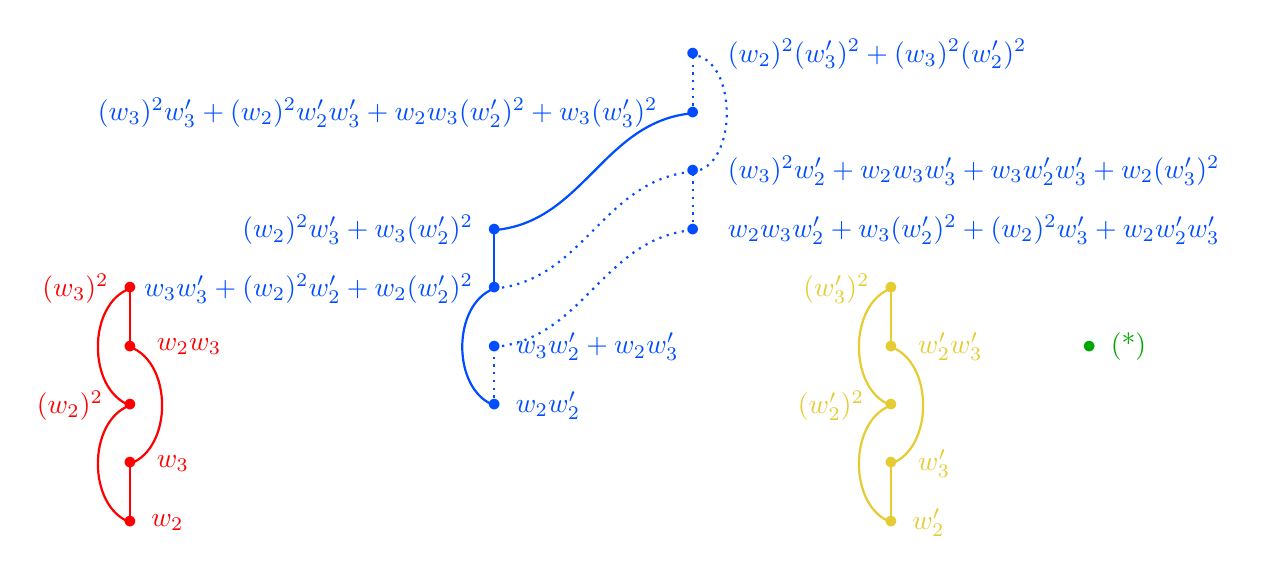
\begin{tikzpicture}[thick,baseline=(m-2-4.south)]
		\matrix (m) [
			matrix of math nodes,
			row sep= 1em,
			column sep=6em,
		]{
			&&& \colorB{\bullet}\\
			&&& \colorB{\bullet}\\
			&&& \colorB{\bullet}\\
			&& \colorB{\bullet} & \colorB{\bullet}\\
			\colorA{\bullet} && \colorB{\bullet} && \colorC{\bullet}\\
		    \colorA{\bullet} && \colorB{\bullet} && \colorC{\bullet} & \colorD{\bullet}\\
			\colorA{\bullet} && \colorB{\bullet} && \colorC{\bullet}\\
			\colorA{\bullet} &&&& \colorC{\bullet}\\
			\colorA{\bullet} &&&& \colorC{\bullet}\\
		};
		\draw[colorA] (m-7-1.center) to [out=200, in=160] (m-9-1.center);
		\draw[colorA] (m-9-1.center) to (m-8-1.center);
		\draw[colorA] (m-5-1.center) to [out=200, in=160] (m-7-1.center);
		\draw[colorA] (m-6-1.center) to (m-5-1.center);
		\draw[colorA] (m-6-1.center) to [out=340, in=20] (m-8-1.center);
		%
		\node[colorA, right=4pt] at (m-9-1) {$w_2$};
		\node[colorA, right=6pt] at (m-8-1) {$w_3$};
		\node[colorA, left=6pt] at (m-7-1) {$(w_2)^2$};
		\node[colorA, right=6pt] at (m-6-1) {$w_2w_3$};
		\node[colorA, left=4pt] at (m-5-1) {$(w_3)^2$};
		%
		\draw[colorB] (m-7-3.center) to [out=160, in=200] (m-5-3.center);
		\draw[colorB, dotted] (m-7-3.center) to (m-6-3.center);
		\draw[colorB, dotted] (m-6-3.center) to [out=5, in=185] (m-4-4.center);
		\draw[colorB] (m-5-3.center) to (m-4-3.center);
		\draw[colorB, dotted] (m-5-3.center) to [out=5, in=185] (m-3-4.center);
		\draw[colorB, dotted] (m-4-4.center) to (m-3-4.center);
		\draw[colorB] (m-4-3.center) to [out=5, in=185] (m-2-4.center);
		\draw[colorB, dotted] (m-2-4.center) to (m-1-4.center);
		\draw[colorB, dotted] (m-3-4.center) to [out=5, in=355] (m-1-4.center);
		%
		\node[colorB, right=4pt] at (m-7-3) {$w_2w'_2$};
		\node[colorB, right=4pt] at (m-6-3) {$w_3w'_2 + w_2w'_3$};
		\node[colorB, left=4pt] at (m-5-3) {$w_3w'_3 + (w_2)^2w'_2 + w_2(w'_2)^2$};
		\node[colorB, left=4pt] at (m-4-3) {$(w_2)^2w'_3 + w_3(w'_2)^2$};
		%
		\node[colorB, right=4pt] at (m-4-4) {$\begin{array}{r}
			w_2w_3w'_2 + w_3(w'_2)^2
			+ (w_2)^2w'_3 + w_2w'_2w'_3
		\end{array}$};
		\node[colorB, right=4pt] at (m-3-4) {$\begin{array}{r}
			(w_3)^2w'_2 + w_2w_3w'_3
			+ w_3w'_2w'_3 + w_2(w'_3)^2
		\end{array}$};
		\node[colorB, left=4pt] at (m-2-4) {$\begin{array}{r}
			(w_3)^2w'_3 + (w_2)^2w'_2w'_3
			+ w_2w_3(w'_2)^2 + w_3(w'_3)^2
		\end{array}$};
		\node[colorB, right=4pt] at (m-1-4) {$\begin{array}{r}
			(w_2)^2(w'_3)^2 + (w_3)^2(w'_2)^2
		\end{array}$};
		%
		\draw[colorC] (m-7-5.center) to [out=200, in=160] (m-9-5.center);
		\draw[colorC] (m-9-5.center) to (m-8-5.center);
		\draw[colorC] (m-5-5.center) to [out=200, in=160] (m-7-5.center);
		\draw[colorC] (m-6-5.center) to (m-5-5.center);
		\draw[colorC] (m-6-5.center) to [out=340, in=20] (m-8-5.center);
		%
		\node[colorC, right=4pt] at (m-9-5) {$w'_2$};
		\node[colorC, right=6pt] at (m-8-5) {$w'_3$};
		\node[colorC, left=6pt] at (m-7-5) {$(w'_2)^2$};
		\node[colorC, right=6pt] at (m-6-5) {$w'_2w'_3$};
		\node[colorC, left=4pt] at (m-5-5) {$(w'_3)^2$};
		%
		\node[colorD, right=4pt] at (m-6-6) {(*)};
	\end{tikzpicture}
\end{equation}
To be consistent with the AHSS computation,
it seems that $w_3w_2' + w_2w'_3$ should be modded out
(is it an obvious consequence of the transgression in LSSS...?)
and the remaing part \colorD{(*)} turns out to be
\begin{equation}
	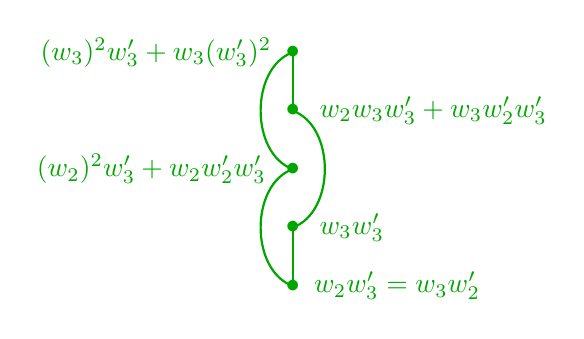
\begin{tikzpicture}[colorD, thick,baseline=(m-2-1.south)]
		\matrix (m) [
			matrix of math nodes,
			row sep= 1em,
			column sep=6em,
		]{
			\bullet\\
		    \bullet\\
			\bullet\\
			\bullet\\
			\bullet\\
		};
		\draw (m-3-1.center) to [out=200, in=160] (m-5-1.center);
		\draw (m-5-1.center) to (m-4-1.center);
		\draw (m-1-1.center) to [out=200, in=160] (m-3-1.center);
		\draw (m-2-1.center) to (m-1-1.center);
		\draw (m-2-1.center) to [out=340, in=20] (m-4-1.center);
		%
		\node[right=4pt] at (m-5-1) {$w_2w'_3 = w_3w'_2$};
		\node[right=6pt] at (m-4-1) {$w_3w'_3$};
		\node[left=6pt] at (m-3-1) {$(w_2)^2w'_3 + w_2w'_2w'_3$};
		\node[right=6pt] at (m-2-1) {$w_2w_3w'_3 + w_3w'_2w'_3$};
		\node[left=4pt] at (m-1-1) {$(w_3)^2w'_3 + w_3(w'_3)^2$};
	\end{tikzpicture}
\end{equation}
and therefore one concludes
\begin{equation}
	\widetilde H^\ast(B\left(\tfrac{SO(4)\times SU(2)}{\bZ_2}\right);\bZ_2)_{\leq 5} = \colorA{J[2]} \oplus \colorC{J[2]} \oplus \colorB{\mathcal{A}_1/\!\!/\mathcal{E}_0[4]} \oplus \colorD{J[5]}.
\end{equation}
This leads to the following Adams chart:
\begin{center}
	\begin{sseqdata}[
		name=M,
		Adams grading,
		classes = fill,
		xrange = {0}{5},
		yrange = {0}{3},
		%,x label = {$t-s$}, y label = {$s$}
	]
		\tower[colorB](4,0)
		\class[white](4,0)
		\class[white](4,0)
		\class[colorA](2,0)
		\class[colorC](2,0)
		\tower[colorA](4,1)
		\tower[colorC](4,1)
		\class[colorD](5,0)
	\end{sseqdata}
	\printpage[name = M,page = 2]
\end{center}
and it indeed seems to be compatible with the AHSS computation.
If the above argument (and beliefs) is correct, then the anomaly should be captured by
\begin{equation}
	w_2w'_3\ (= w_3w'_2).
\end{equation}

\subsection{Seiberg dual}
The dual theory is $SO(2)$ gauge theory with $N_f = 2$ flavors, and the fermions are charged under
\begin{equation}
	\frac{SO(2)\times SU(2)}{\bZ_2}
	=
	U(2)
\end{equation}
Its spin bordism is known, and the relevant group turns out to be trivial:
\begin{equation}
	\Omega_5^{\mathrm{spin}}\big(BU(2)\big) = 0.
\end{equation}
This means there is no anomaly for fermions on the dual side,
and thus the $B\beta E$ anomaly cannot be canceled by fermions.

\newpage

\section{'t Hooft-Polyakov monopole argument}
For an $SU(2)$ gauge theory Higgssed by an adjoint ($\bm{3}$, spin-$1$, isovector) scalar,
the gauge group is broken down to $U(1)$, and correspondingly it accommodates topological solitons (monopoles):
\begin{equation*}
	\pi_2\left(
		\dfrac{SU(2)}{U(1)}
	\right) = \bZ.
\end{equation*}
In the presence of (additional) fermions, this monopole might acquire non-trivial charge under
spacetime-Lorentz or flavor symmetries, depending on the representation of the fermions under $SU(2)$ gauge symmetry:
\begin{equation*}
	\begin{tabular}{c||cccc}
		fermion gauge rep. & number of zero-modes & spin of zero-modes& spin of monopole\\
		\hline
		$\bm{2}$ & $1$ & $0$ & $0$\\
		$\bm{3}$ & $2$ & $\tfrac{1}{2}$\\
		$\bm{4}$ & $4$ & $0\oplus 1$ & $\tfrac{1}{2}$\\
	\end{tabular}
\end{equation*}
The numbers of zero-modes can be computed from the Callias index theorem\cite{Callias:1977kg}.

According to \cite{Wang:2018qoy},
there is $w_2(TM_4)\beta w_2(SU(2)_{\text{gauge}})$ anomaly for a fermion in $\bm{4}$ charged under
\begin{equation*}
	\dfrac{Spin(4)_{\text{spacetime}} \times SU(2)_{\text{gauge}}}{\bZ_2},
\end{equation*}
which incarnates in the IR as an ill-definition of the effective interaction $w_2(TM) c_1(U(1)_{\text{gauge}})$,
emerging after integrating out the fermion which obtained mass through Yukawa coupling.
This effective interaction term should arise in order to make the monopole a fermion
(\textit{i.e.}\,spinor representation of $Spin(4)_{\text{spacetime}}$),
but is not well-defined without a trivialization of $w_2(TM_4)$ or equivalently a spin structure.

This situation looks quite similar to our problem where the fermions are charged under
\begin{equation*}
	\dfrac{SO(4)_{\text{gauge}} \times SU(2)_{\text{flavor}}}{\bZ_2}.
\end{equation*}
Since fermions are in the fundamental representation of the flavor symmetry,
breaking $SU(2)_{\text{flavor}}$ to $U(1)_{\text{flavor}}$ gives rise to
a monopole in the spinor representation this time of the $SO(4)_{\text{gauge}}$\cite{Harvey:1996ur}.
Therefore by the same logic, one can deduce that there should be
$w_2(SO(4)_{\text{gauge}})\beta w_2(SU(2)_{\text{flavor}})$ anomaly in the first place, as desired.

Also, one should be able to generalize this whole argument to the case of fermions charged under
\begin{equation*}
	\dfrac{SO(2n_c)_{\text{gauge}} \times SU(2n_f)_{\text{flavor}}}{\bZ_2}
\end{equation*}
by breaking $SU(2n_f)_{\text{flavor}}$ to $SO(2n_f)_{\text{flavor}}$,
where we have monopoles characterized by
\begin{equation*}
	\pi_2\left(
		\dfrac{SU(2n_f)}{SO(2n_f)}
	\right)
	=
	\left\{
		\begin{array}{cl}
			\bZ_2 & (n_f \geq 2)\\
			\bZ & (n_f = 1)
		\end{array}
	\right..
\end{equation*}

\newpage

\section{misc}

\subsection{$\bZ_4$ 1-form symmetry}
According to \cite[Appendix C.3]{Clement2002} and \cite[Eq.\,(6.3)]{Wan:2018bns}, it seems that we have
\begin{equation}
	\begin{array}{ccc}
		E^2_{p,q}=H_p\big(K(\bZ_4,2);\Omega_q^{\text{spin}}\big) && \widetilde\Omega_{p+q}^{\text{spin}}(K(\bZ_4,2))\vspace{4mm}\\
		\begin{array}{c|c:cccccccccccc}
			6  &&&&&& \\
			5  & \cellcolor{lightyellow} & \hphantom{\bZ_2} & \hphantom{\bZ_2} & \hphantom{\bZ_2} & \hphantom{\bZ_2} & \hphantom{\bZ_2} \\
			4  & \bZ & \cellcolor{lightyellow} & \ast && \ast & \ast & \ast\\
			3  &  && \cellcolor{lightyellow} &&&\\
			2  & \bZ_2 &  & \red{\fbox{\black{$\bZ_2$}}} & \Blue{\fbox{\black{$\bZ_2$}}}\cellcolor{lightyellow} & \ast & \ast & \ast\\
			1  & \bZ_2 && \red{\dbox{\black{$\bZ_2$}}} & \Blue{\dbox{\black{$\bZ_2$}}} & \red{\fbox{\black{$\bZ_2$}}}\cellcolor{lightyellow} & \Blue{\fbox{\black{$\bZ_2$}}} & \ast\\
			0 & \bZ &  & \bZ_4 &  & \red{\dbox{\black{$\bZ_8$}}} & \Blue{\dbox{\black{$\bZ_2$}}} \cellcolor{lightyellow} & \ast\\
			\hline
			& 0 & 1 & 2 & 3 & 4 & 5 & 6 \\
		\end{array}
		& \quad\longrightarrow & 
		\begin{array}{c|c}
			6  & \ast\\
			5  & \cellcolor{lightyellow}\\
			4  & \bZ_4\\
			3  & \\
			2  & \bZ_4\\
			1  & \\
			0 & \\
			\hline\\
		\end{array}
	\end{array}
\end{equation}

\subsection{$\bZ_2\times \bZ_2$ 1-form symmetry}
Exploiting the fact that $K(\bZ_2\times \bZ_2, 2) = K(\bZ_2, 2) \times K(\bZ_2, 2)$,
it seems that we have
\begin{equation}
	\begin{array}{ccc}
		E^2_{p,q}=H_p\big(K(\bZ_2\times \bZ_2,2);\Omega_q^{\text{spin}}\big)
		&& \widetilde\Omega_{p+q}^{\text{spin}}(K(\bZ_2\times \bZ_2,2))\vspace{4mm}\\
		\begin{array}{c|c:cccccccccccc}
			6  &&&&&& \\
			5  & \cellcolor{lightyellow} & \hphantom{\bZ_2} & \hphantom{\bZ_2} & \hphantom{\bZ_2} & \hphantom{\bZ_2} & \hphantom{\bZ_2} \\
			4  & \bZ & \cellcolor{lightyellow} & \ast && \ast & \ast & \ast\\
			3  &  && \cellcolor{lightyellow} &&&\\
			2  & \bZ_2 &  & \red{\fbox{\black{$\bZ_2^{\oplus 2}$}}} & \Blue{\fbox{\black{$\bZ_2^{\oplus 2}$}}}\cellcolor{lightyellow} & \ast & \ast & \ast\\
			1  & \bZ_2 && \red{\dbox{\black{$\bZ_2^{\oplus 2}$}}} & \Blue{\dbox{\black{$\bZ_2^{\oplus 2}$}}} & \green{\fbox{\red{\fbox{\black{$\bZ_2^{\oplus 3}$}}}}}\cellcolor{lightyellow} & \Blue{\fbox{\black{$\bZ_2^{\oplus 6}$}}} & \ast\\
			0 & \bZ &  & \bZ_2^{\oplus 2} &  & \red{\dbox{\black{$\bZ_4^{\oplus 2}\oplus \bZ_2$}}} & \Blue{\dbox{\black{$\bZ_2^{\oplus 3}$}}} \cellcolor{lightyellow} & \green{\fbox{\black{$\ast$}}}\\
			\hline
			& 0 & 1 & 2 & 3 & 4 & 5 & 6 \\
		\end{array}
		& \quad\longrightarrow & 
		\begin{array}{c|c}
			6  & \ast\\
			5  & \bZ_2\cellcolor{lightyellow}\\
			4  & \bZ_2^{\oplus 3}\\
			3  & \\
			2  & \bZ_2^{\oplus 2}\\
			1  & \\
			0 & \\
			\hline\\
		\end{array}
	\end{array}
\end{equation}
The $\bZ$ homology of $K(\bZ_2, 2)$ is again read off from \cite{Clement2002},
while the $\bZ_2$ (co)homology is known \cite{Serre1953} to be
\begin{equation*}
	H^\ast(K(\bZ_2,2);\bZ_2)
	=
	\bZ_2[x_2, Sq^1 x_2, Sq^2Sq^1 x_2, \cdots].
\end{equation*}

\newpage


\bibliographystyle{ytphys}
\baselineskip=.95\baselineskip
\bibliography{ref}

\end{document}